\subsection{Regler}
\begin{frame}{Transformations Regler}
	Transformationer som har mulighed for at gøre en fabriks konfiguration bedre
	\begin{itemize}
		\item Anti-Serialize
		\item Parallelize
		\item Swap		
	\end{itemize}
\end{frame}


% De gør et system bedre.
% Eksempel på hvad de enkelte regler gør.
\subsection{Forbedringer}
\begin{frame}{Multiple Recipe Anti-Serialize}
	\begin{itemize}
		\item Vi anti-serialisere flere recipes ud på engang
		\item Dette er godt hvis vi har en mængde moduler som bedre kan løse et delmængde af recipes, men ikke resten
	\end{itemize}
\end{frame}

\begin{frame} {Multiple Recipe Anti-Serialize}
	\begin{figure}
		\centering
		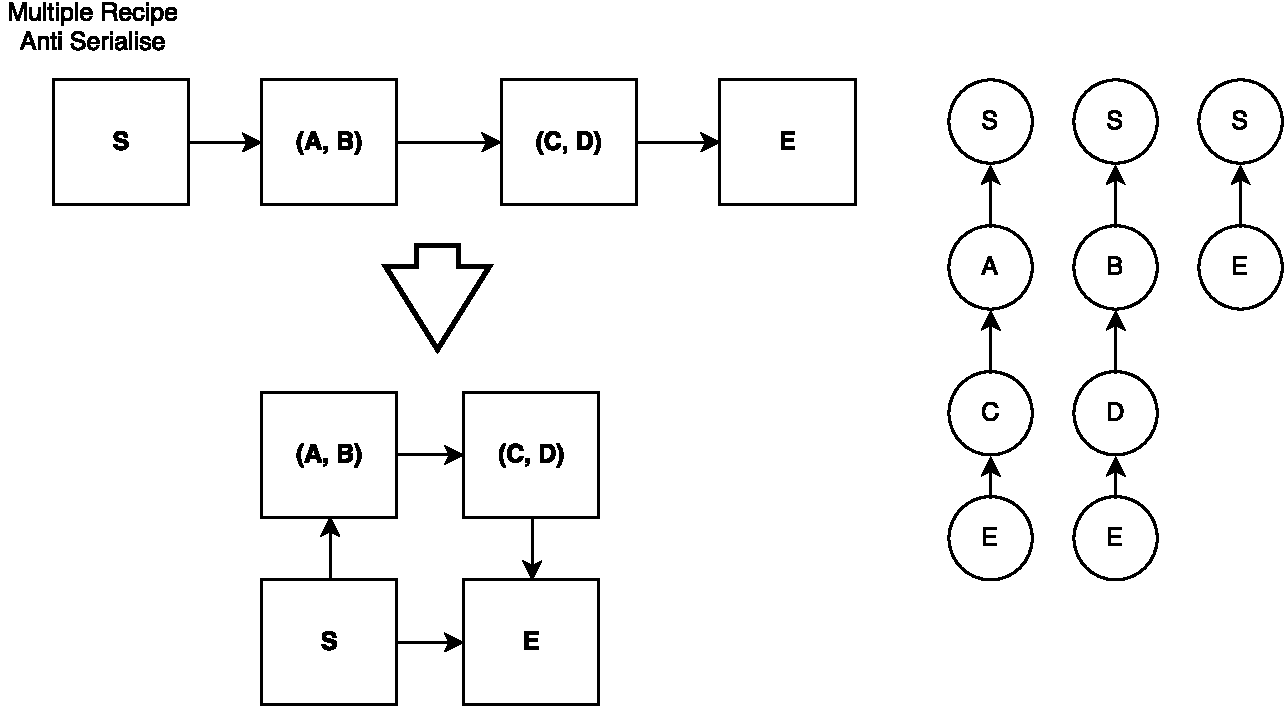
\includegraphics[width=1\textwidth]{figures/mras.pdf}
	\end{figure}
\end{frame}

\begin{frame}{Mere Robust Parallelize}
	\begin{itemize}
		\item Lige nu skal der være et 1 til 1 forhold mellem hvad de moduler vi gerne vil paralellisere kan og dem som vi bruger til at parallelisere med
		\item Vi gerne være i stand til at parallelisere en mængde af moduler så længe den mængde kan udføre det samme arbejde i den række den række følge, som den mængde vi parallelisere ud fra
	\end{itemize}
\end{frame}

\begin{frame} {Mere Robust Parallelize}
	\begin{figure}
		\centering
		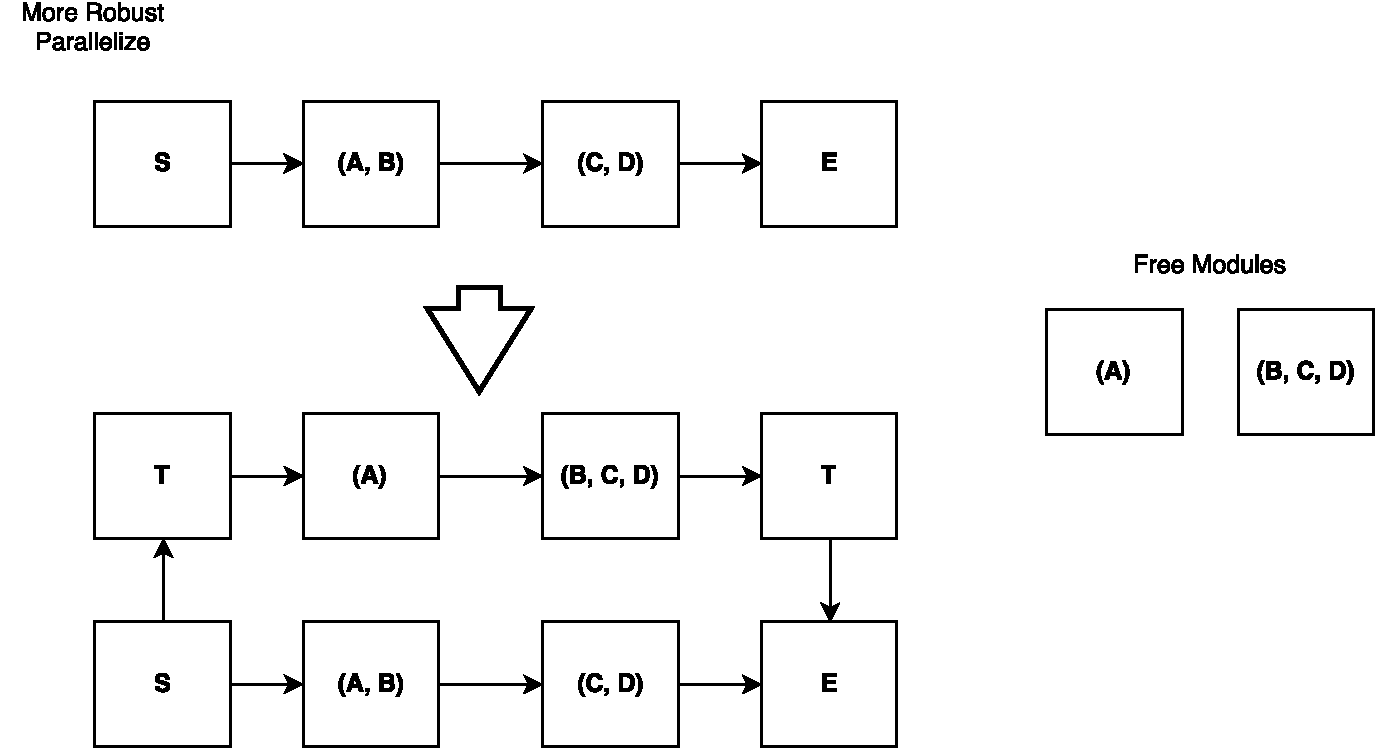
\includegraphics[width=1\textwidth]{figures/mrpara.pdf}
	\end{figure}
\end{frame}

\begin{frame}{Multiple Swap og Safe Swap}
	\begin{itemize}
		\item \textbf{Multiple Swap}: Igen være i stand til at swappe en mængde moduler ind eller ud, med en anden mængde moduler som er i stand til det samme arbejde i samme rækkefølge
		\item \textbf{Safe Swap}: Være i stand til at swappe moduler rundt i en konfiguration, hvor det stadigvæk er muligt at udføre recipes.
	\end{itemize}
\end{frame}



\section{Tabu Search}
\begin{frame} {Tabu Search}
	\begin{itemize}
		\item Tabu er en form for local search, men med hukommelse om hvad den tidliger har gjort.
		\item Hvorfor bruger vi Tabu Search?
		\item Hvorfor ikke en genetisk algorithme
	\end{itemize}
\end{frame}

\begin{frame} {Tabu Search}
	Hvordan fungere vores tabu search?
	\begin{itemize}
		\item Vi kan bruge vores transformations regler til at finde naboer
		\item Topologisk Sort af recipes til at finde $C_{naive}$
		\item Bruger langtidshukommelse til at gå tilbage til tidligere besøgte konfigurationer
		\item Bruger korttidshukommelse til at restriktere hvilke naboer vi må tage.
		\item Vi vælger at fase vores regler på forskellige tidspunkter for potentielt bedre søgninger
		\begin{itemize}
			\item Start: Mest sandsynelig at Anti-Serialisere
			\item Midt: Mest sandsynelig at Parallelisere
			\item Slut: Mest sandsynelig at Swappe
		\end{itemize}
	\end{itemize}
\end{frame}

\begin{frame}{Bedre Heuristikker til Tabu Search}
	\begin{itemize}
		\item Bedre håndtering af langtidshukommelse
		\begin{itemize}
			\item Bedre udvælgelse af hvornår noget skal i langtidshukommelse
			\item Måske ikke lade searchen tage en gammel route med det samme igen efter man er gået tilbage til et punkt i langtidshukommelsen.
		\end{itemize}
		\item Beskrive konfigurationer med flere attributer
		\begin{itemize}
			\item Beskriv sektioner i en konfiguration hvori ændrelser kan gøres til en tabu hvis de når et kriterie
		\end{itemize}
	\end{itemize}
\end{frame}

% Hvorfor Tabu Search
% Kobling til Regler 
% Andre Heuristiker vi kunne have brugt og forbedringer.

\section{Konklusion}
\begin{frame}{Konklusion}
	Så hvad har vi lavet?
	\begin{itemize}
		\item En UPPAAL model baseret på virkelige modulere fabrikker, som korrekt kan simulere dem
		\item Opsat regler for transformationer som kan har mulighed for at forbedre en konfiguration
		\item Implemeteret nævnte regler i en tabu search som er i stand til at søge efter en optimal konfiguration
	\end{itemize}
\end{frame}

\begin{frame}{Konklusion}
	\textit{How may we, given some order of items and set of available modules, be able to generate a factory configuration which has the fastest schedule of any other candidate configuration?}
	\begin{itemize}
		\item Løste vi vores problem?
	\end{itemize}
\end{frame}



% Kort om at vi løser problemet
